\documentclass[c]{beamer}
%\documentclass[c,aspectratio=1610]{beamer}
\mode<presentation>
{
  \usetheme[progressbar=frametitle]{metropolis}       % or try default, Darmstadt, Warsaw, Darmstadt ,Berkeley,...
  \usecolortheme{default} % or try albatross, beaver, crane,whale,orchid,spruce,...
  \usefonttheme{serif}    % or try default, structurebold,serif ...
  \setbeamertemplate{navigation symbols}{}
  \setbeamertemplate{caption}[numbered]
  \setbeamercovered{transparent}
} 


\usepackage[utf8]{inputenc}
\usepackage[brazil]{babel}
\usepackage[brazilian,hyperpageref]{backref}
\usefonttheme{serif}
\usepackage{ebgaramond-maths}
\usepackage{amsmath,amssymb}
\usepackage{graphicx}
\usepackage{float}
\usepackage{caption}
\usepackage{subcaption}
\captionsetup[figure]{labelfont=sc}
 \usepackage{multicol}
\usepackage{verbatim}


\title{{\sc Introdução ao \LaTeX}}
\subtitle{Módulo 3: Apresentações de slides, Referências e outras técnicas.}
\date{\today}
\author{	{\large XI Semana Acadêmica da Física}\\
	Geferson {\sc Lucatelli}\inst{1}\footnote{\texttt{gefersonlucatelli@gmail.com}},
	Fernanda Vanucci {\sc Sica}\inst{1}\footnote{\texttt{fervanucci@gmail.com\\[0.5cm]}}}
\institute{{\Large Universidade Federal do Rio Grande} \\[0.3cm]
	{\inst{1}\large Instituto de Matemática, Estatística e Física
	}}
\titlegraphic{\hfill
	
\includegraphics[height=1.5cm]{images/furg.png}\\[2.5cm]{
\hspace*{8cm}
\includegraphics[height=1.5cm]{images/imef2.png}}
\hspace*{7.8cm}
\includegraphics[height=2.5cm]{images/safis2018.pdf}
}

\bibliographystyle{apalike}
\setbeamertemplate{section in toc}{\hspace*{1em}\inserttocsectionnumber.~\inserttocsection\par}
\setbeamertemplate{subsection in toc}{\hspace*{2em}\inserttocsectionnumber.\inserttocsubsectionnumber.~\inserttocsubsection\par}
\setbeamercovered{invisible}
\newcommand{\linesH}[1]{\rule{\linewidth}{#1}}
\begin{document}
\maketitle


{\fontsize{9pt}{10.0}\selectfont

\begin{frame}{\sc Sumário}
	\begin{multicols}{2}
			\tableofcontents
	\end{multicols}
%  \setbeamertemplate{section in toc}[sections numbered]
%  \tableofcontents[section,subsection]
% \tableofcontents[hideallsubsubsections]
%   \tableofcontents[hideallsubsubsections]
\end{frame}
}
%%%%%%%%%%%%%%%%%%%%%%%%%%%%
%
%\begin{frame}
%	\begin{center}
%		{\Huge Parte 2}
%	\end{center}
%\end{frame}

{\fontsize{10pt}{10.0}\selectfont

\section{Apresentações Beamer}
\subsection{Estrutura}
\plain{Como criar apresentações de slides utilizando o \LaTeX?}
\plain{Através da classe \texttt{beamer} !}

\begin{frame}[fragile]{{\sc Estrutura do }\texttt{beamer}}
	\begin{itemize}
		\setlength\itemsep{0.3cm}
  \item Em \LaTeX\ é possível criar apresentações de uma forma simples e de qualidade, com o pacote \verb| beamer |. Basta definir como classe:\\
  \begin{verbatim}
	\documentclass[opções]{beamer}
  \end{verbatim}
  \item algumas opções são tamanho \verb|8pt,9pt,10pt,11pt,...|;
  \item o uso de pacotes é idêntico às outras classes \verb| book, article | etc.;
  \item informações básicas sobre o documento são:\\
\begin{verbatim}
  \title{}
  \subtitle{}
  \date[]{}
  \author{}
  \institute{}
  \logo{}
  \end{verbatim}
	\end{itemize}
\end{frame}



\begin{frame}[fragile]{{\sc Estrutura do }\texttt{beamer}}
	\begin{itemize}
		\setlength\itemsep{0.3cm}
		\item da mesma forma que outras classes, tudo o que estiver entre 
		\begin{center}
			\verb| \begin{document} |\\
			.\\
			.\\
			.\\
			\verb| \end{document} |
		\end{center}
		constitui-rá tudo o que estiver escrito nos \emph{frames}: textos, listas, tabelas, figuras, equações etc;
		\item um frame é uma página da apresentação, e é construído por:\\
		\verb|\begin{frame}[opções]{título}{subtítulo}|\\
		\verb|\end{frame}|
		\item exemplo de opções: 
		\begin{itemize}
			\item  \verb|fragile|, usado para \emph{macros}, como o \verb|verbatim|;\\
			\item \verb|b|, \verb|c| ou \verb|t|, posição do texto no frame (\verb|b| este frame);
		\end{itemize}
	\end{itemize}
\end{frame}






\begin{frame}[fragile]{{\sc Estrutura do }\texttt{beamer}}
	\begin{itemize}
		\setlength\itemsep{0.3cm}
		\item para se criar o sumário da apresentação, crie um frame e insira o comando \verb|\tableofcontents| da seguinte forma:
        \begin{verbatim}
		    \begin{frame}{Sumário}
		    \tableofcontents
		    \end{frame}|
        \end{verbatim}
		\item se caso o sumário for muito grande e não couber no frame, crie duas colunas (a seguir) ou use o comando 
		\verb|{\fontsize{10pt}{10.0}\selectfont frame do sumário aqui }|;
	\end{itemize}
\end{frame}

\subsection{Ambientes do \texttt{beamer}}
\plain{Vejamos agora alguns ambientes utilizados no \texttt{beamer}}

\begin{frame}[fragile]{{\sc Blocos}}
	\begin{itemize}
		\setlength\itemsep{0.3cm}
		\item ambientes muito utilizados nos beamers são: \verb|itemize|, \verb|enumerate|, \verb|description|;
		\item outros ambientes são os \verb|blocos|: \verb|block|, \verb|alertblock|, \verb|exampleblock|, ...
	\end{itemize}
\begin{figure}[h]
	\centering
	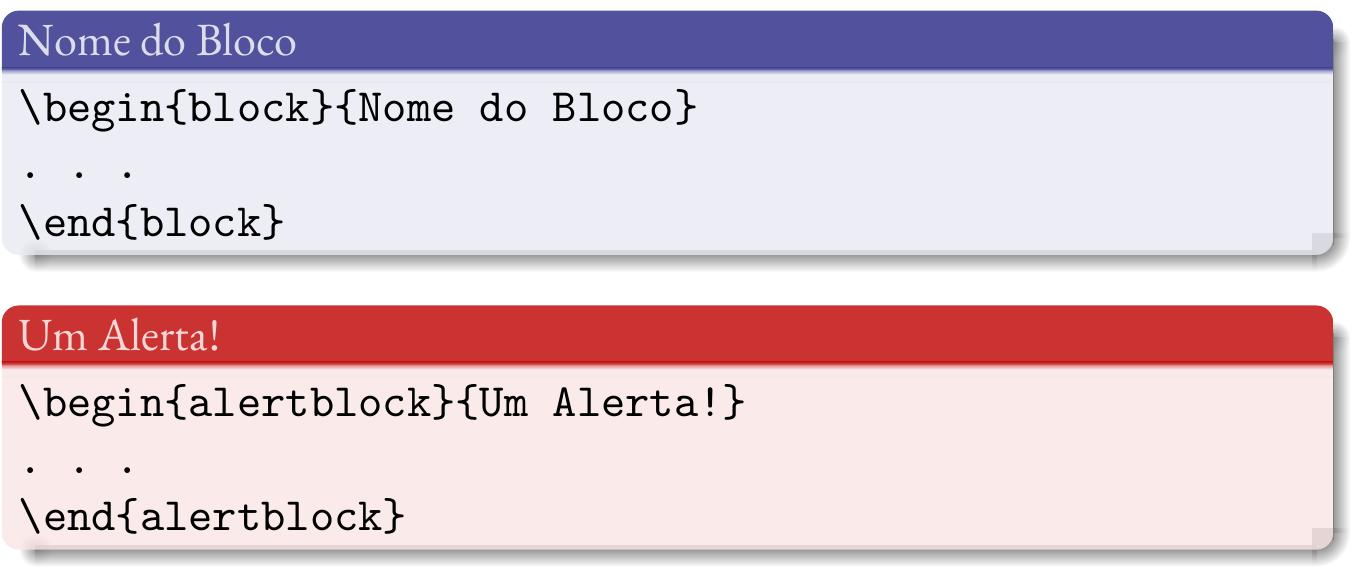
\includegraphics[width=0.99\textwidth]{images/blocks_1.jpg}
\end{figure}
\end{frame}




\begin{frame}[fragile]{\sc Colunas}
	\begin{itemize}
		\setlength\itemsep{0.3cm}
		\item dividir um frame em colunas pode ser bastante útil;
		\item para criá-las basta usar:
		%
		\begin{columns}
			\begin{column}{5cm}
				
				\begin{verbatim}
				\begin{columns}
				\begin{column}[t]{tamanho}
				Criando colunas.
				Duas colunas.
				\end{column}
				\end{verbatim}
				
			\end{column}
			
			\begin{column}{5cm}
				
				\begin{verbatim}     
				\begin{column}[t]{tamanho}
				Tamanho define a largura 
				das colunas. 
				\end{column}
				\end{columns}
				\end{verbatim}
				
			\end{column}
			
		\end{columns}
		\item em uma coluna podemos ter um texto e na outra uma figura (exercício).
	\end{itemize}
\end{frame}

\begin{frame}[fragile]{\sc Colunas - Exercício}
	\begin{columns}
		
		\begin{column}[t]{6cm}
			\begin{figure}[b]
				\centering
				\includegraphics[scale=0.18]{images/NGC_5371.jpg}
				\caption{NGC 5371 - Galáxia espiral barrada, localizada a $\sim$ 100 milhões de anos luz da Terra, 
					na constelação de  Canes Venatici.}
				\label{mod_3_ex_1}
			\end{figure}
			
		\end{column}
		
		
		\begin{column}[t]{6cm}
\begin{figure}[h]
	\centering
	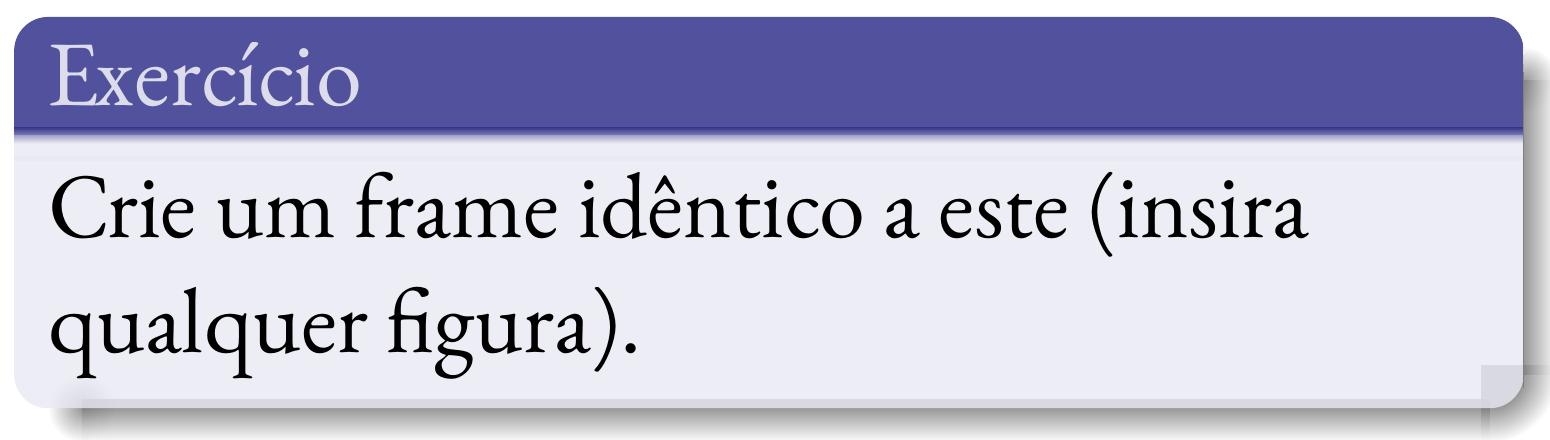
\includegraphics[width=0.99\textwidth]{images/blocks_2.jpg}
\end{figure}
			
			\begin{itemize}
				\item crie duas colunas com 6cm cada;
				\item insira uma figura na coluna esquerda; 
				\item crie um bloco;
				\item faça uma lista qualquer;
			\end{itemize}
			
		\end{column}
		
	\end{columns}
	
\end{frame}


{\fontsize{8pt}{7.0}\selectfont
\begin{frame}[fragile]{\sc Colunas - Exercício}
\begin{verbatim}
\begin{columns}

\begin{column}[t]{6cm}
\begin{figure}[b]
\centering
\includegraphics[scale=0.18]{NGC_5371.jpg}
\caption{NGC 5371 - Galáxia espiral barrada, 
localizada a $\sim$ 100 milhões de anos luz da Terra, 
na constelação de  Canes Venatici.}
\label{mod_3_ex_1}
\end{figure}
\end{column}

\begin{column}[t]{6cm}
\begin{block}{Exercício}
Crie um frame idêntico a este (insira qualquer figura).
\end{block}
\begin{itemize}
\item crie duas colunas com 6cm cada;
\item insira uma figura na coluna esquerda; 
\item crie um bloco;
\item faça uma lista qualquer;
\end{itemize}
\end{column}

\end{columns}
\end{verbatim}
\end{frame}
}


\begin{frame}[fragile]{Temas}
	\begin{itemize}
		\setlength\itemsep{0.3cm}
		\item vários modelos de \emph{beamers} estão disponíveis para utilização;
		\item para isso, modificamos o tema com:\\
		\verb|\usetheme{}| - modifica a estrutura do tema;\\
		\verb|\usecolortheme{}| - modifica a cor do tema;\\
		\verb|\usefonttheme{}| - modifica a fonte do tema
		\item exemplos destes temas são: \verb|\usetheme{Darmstadt}|, \verb|\usecolortheme{orchid}|, \verb|\usefonttheme{serif}|;
		%   \item outras modificações são como a utilizada no exercício, \verb|\setbeamercovered{transparent}|, que deixa também objetos transparentes aos logos nesta 
		%   apresentação;
	\end{itemize}
\end{frame}



\begin{frame}[fragile]{\sc Temas}
\begin{figure}[h]
	\centering
	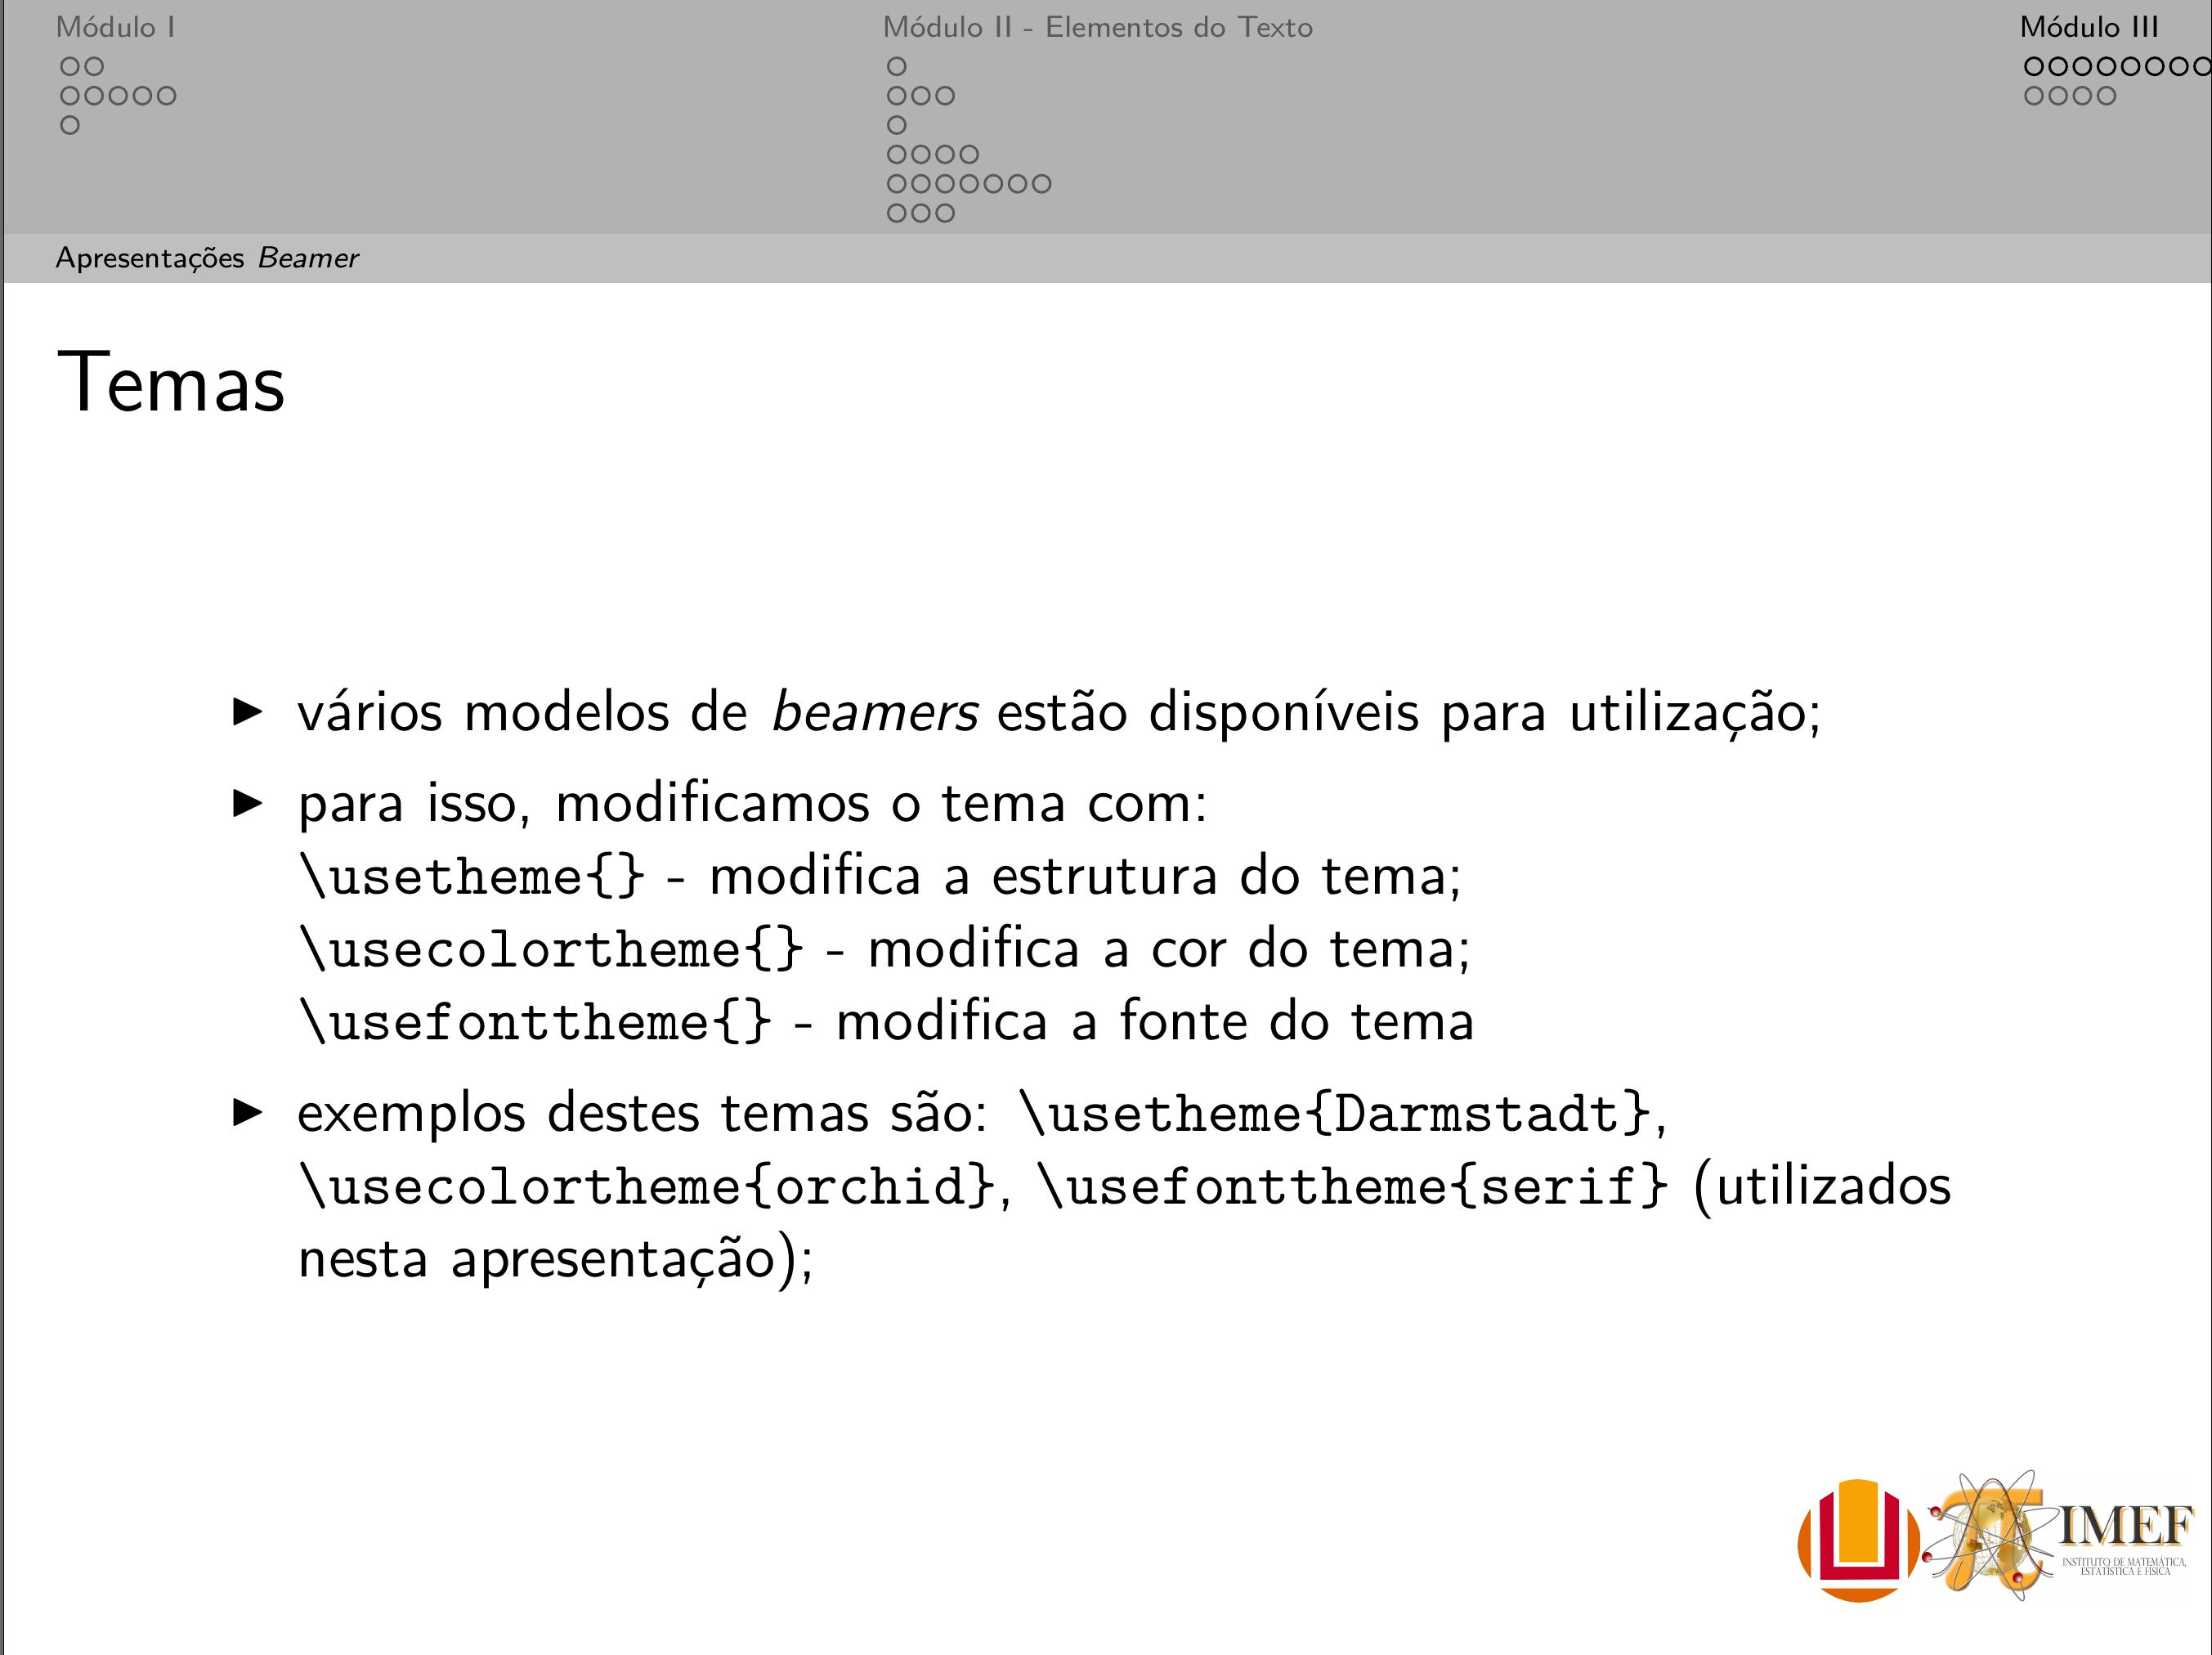
\includegraphics[width=0.40\textwidth]{images/beamer_sze_seau.jpg}
	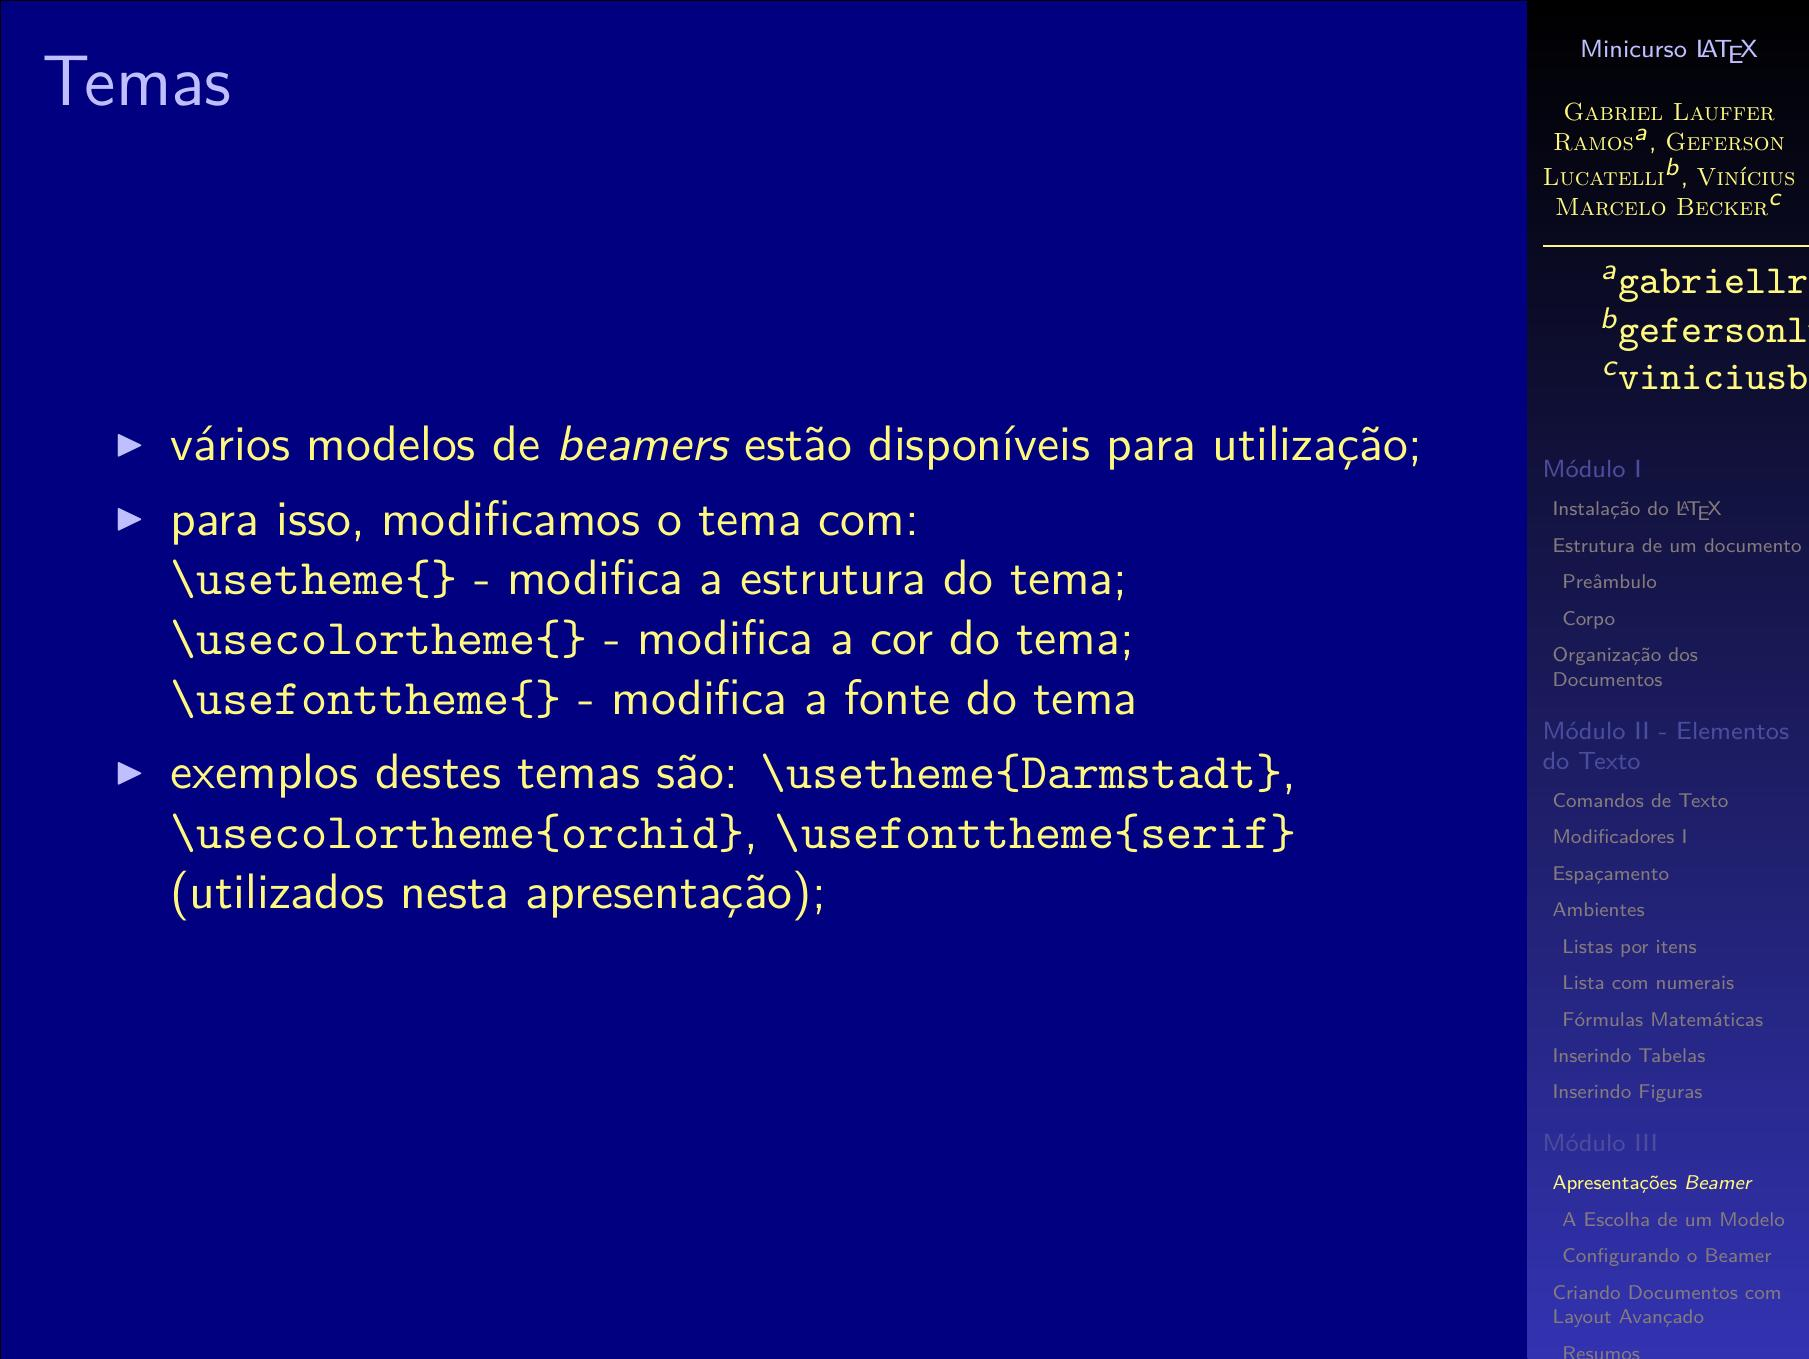
\includegraphics[width=0.40\textwidth]{images/beamer_marb_alb.jpg}\\
	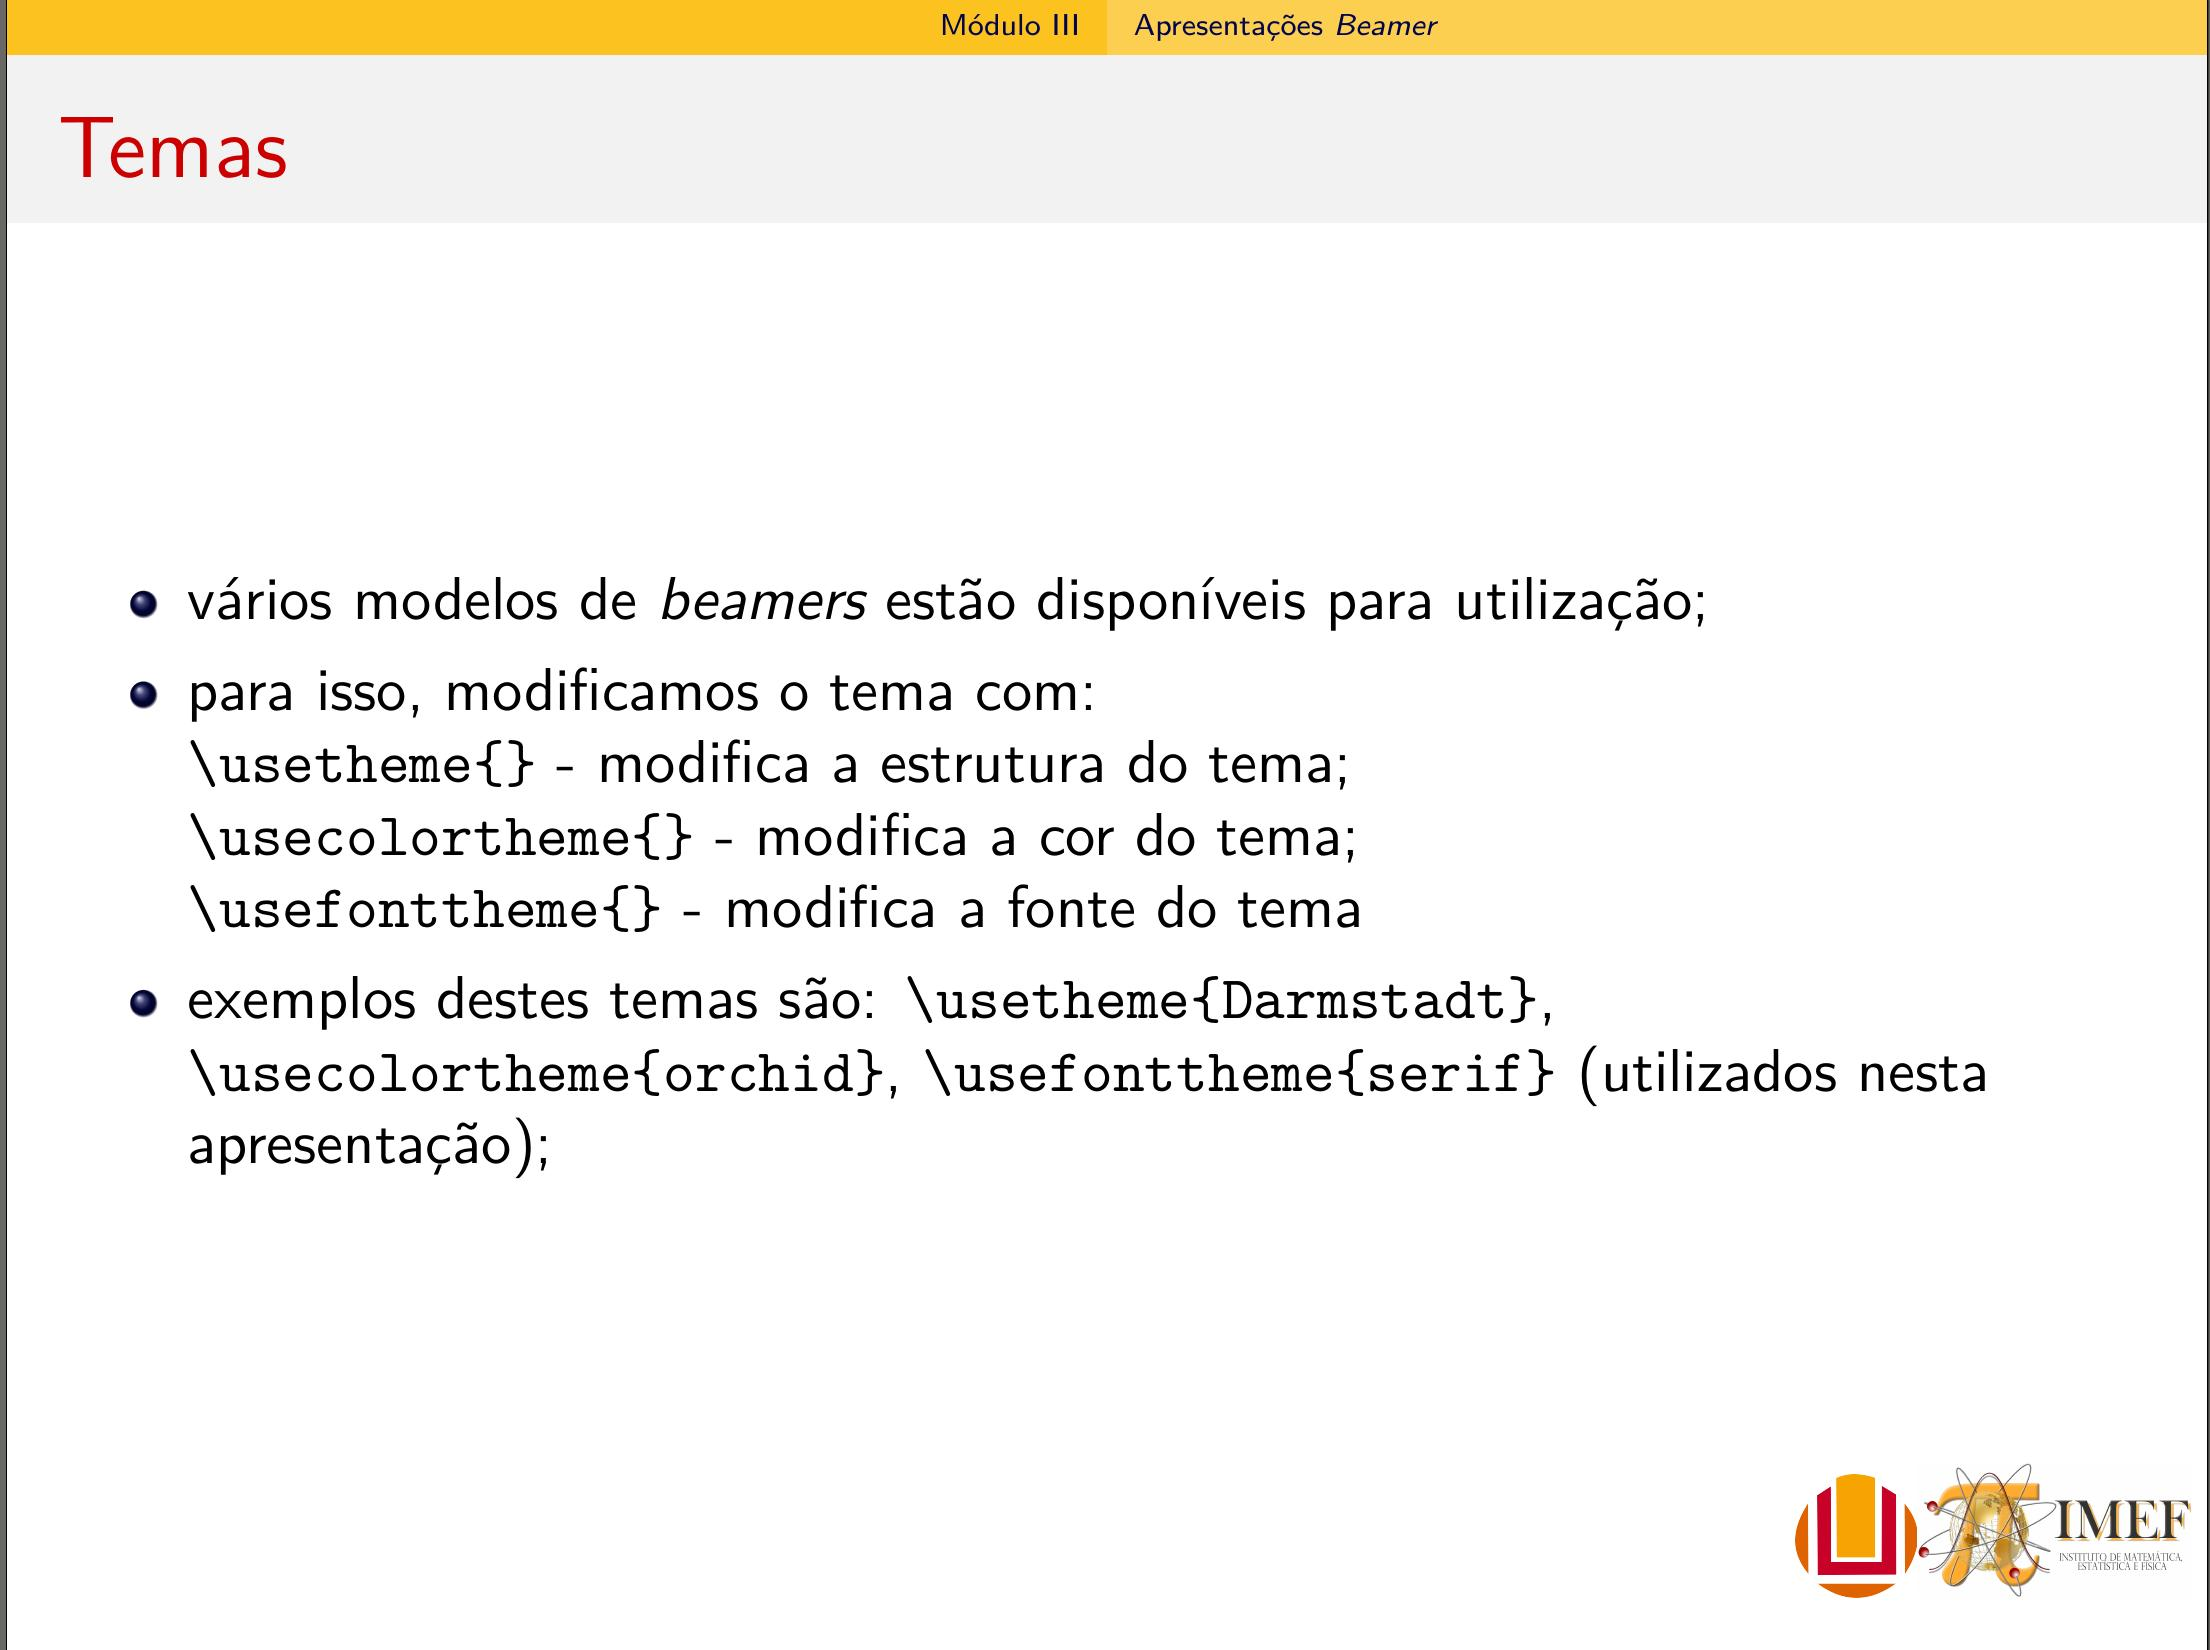
\includegraphics[width=0.40\textwidth]{images/beamer_cambr_crane.jpg}
	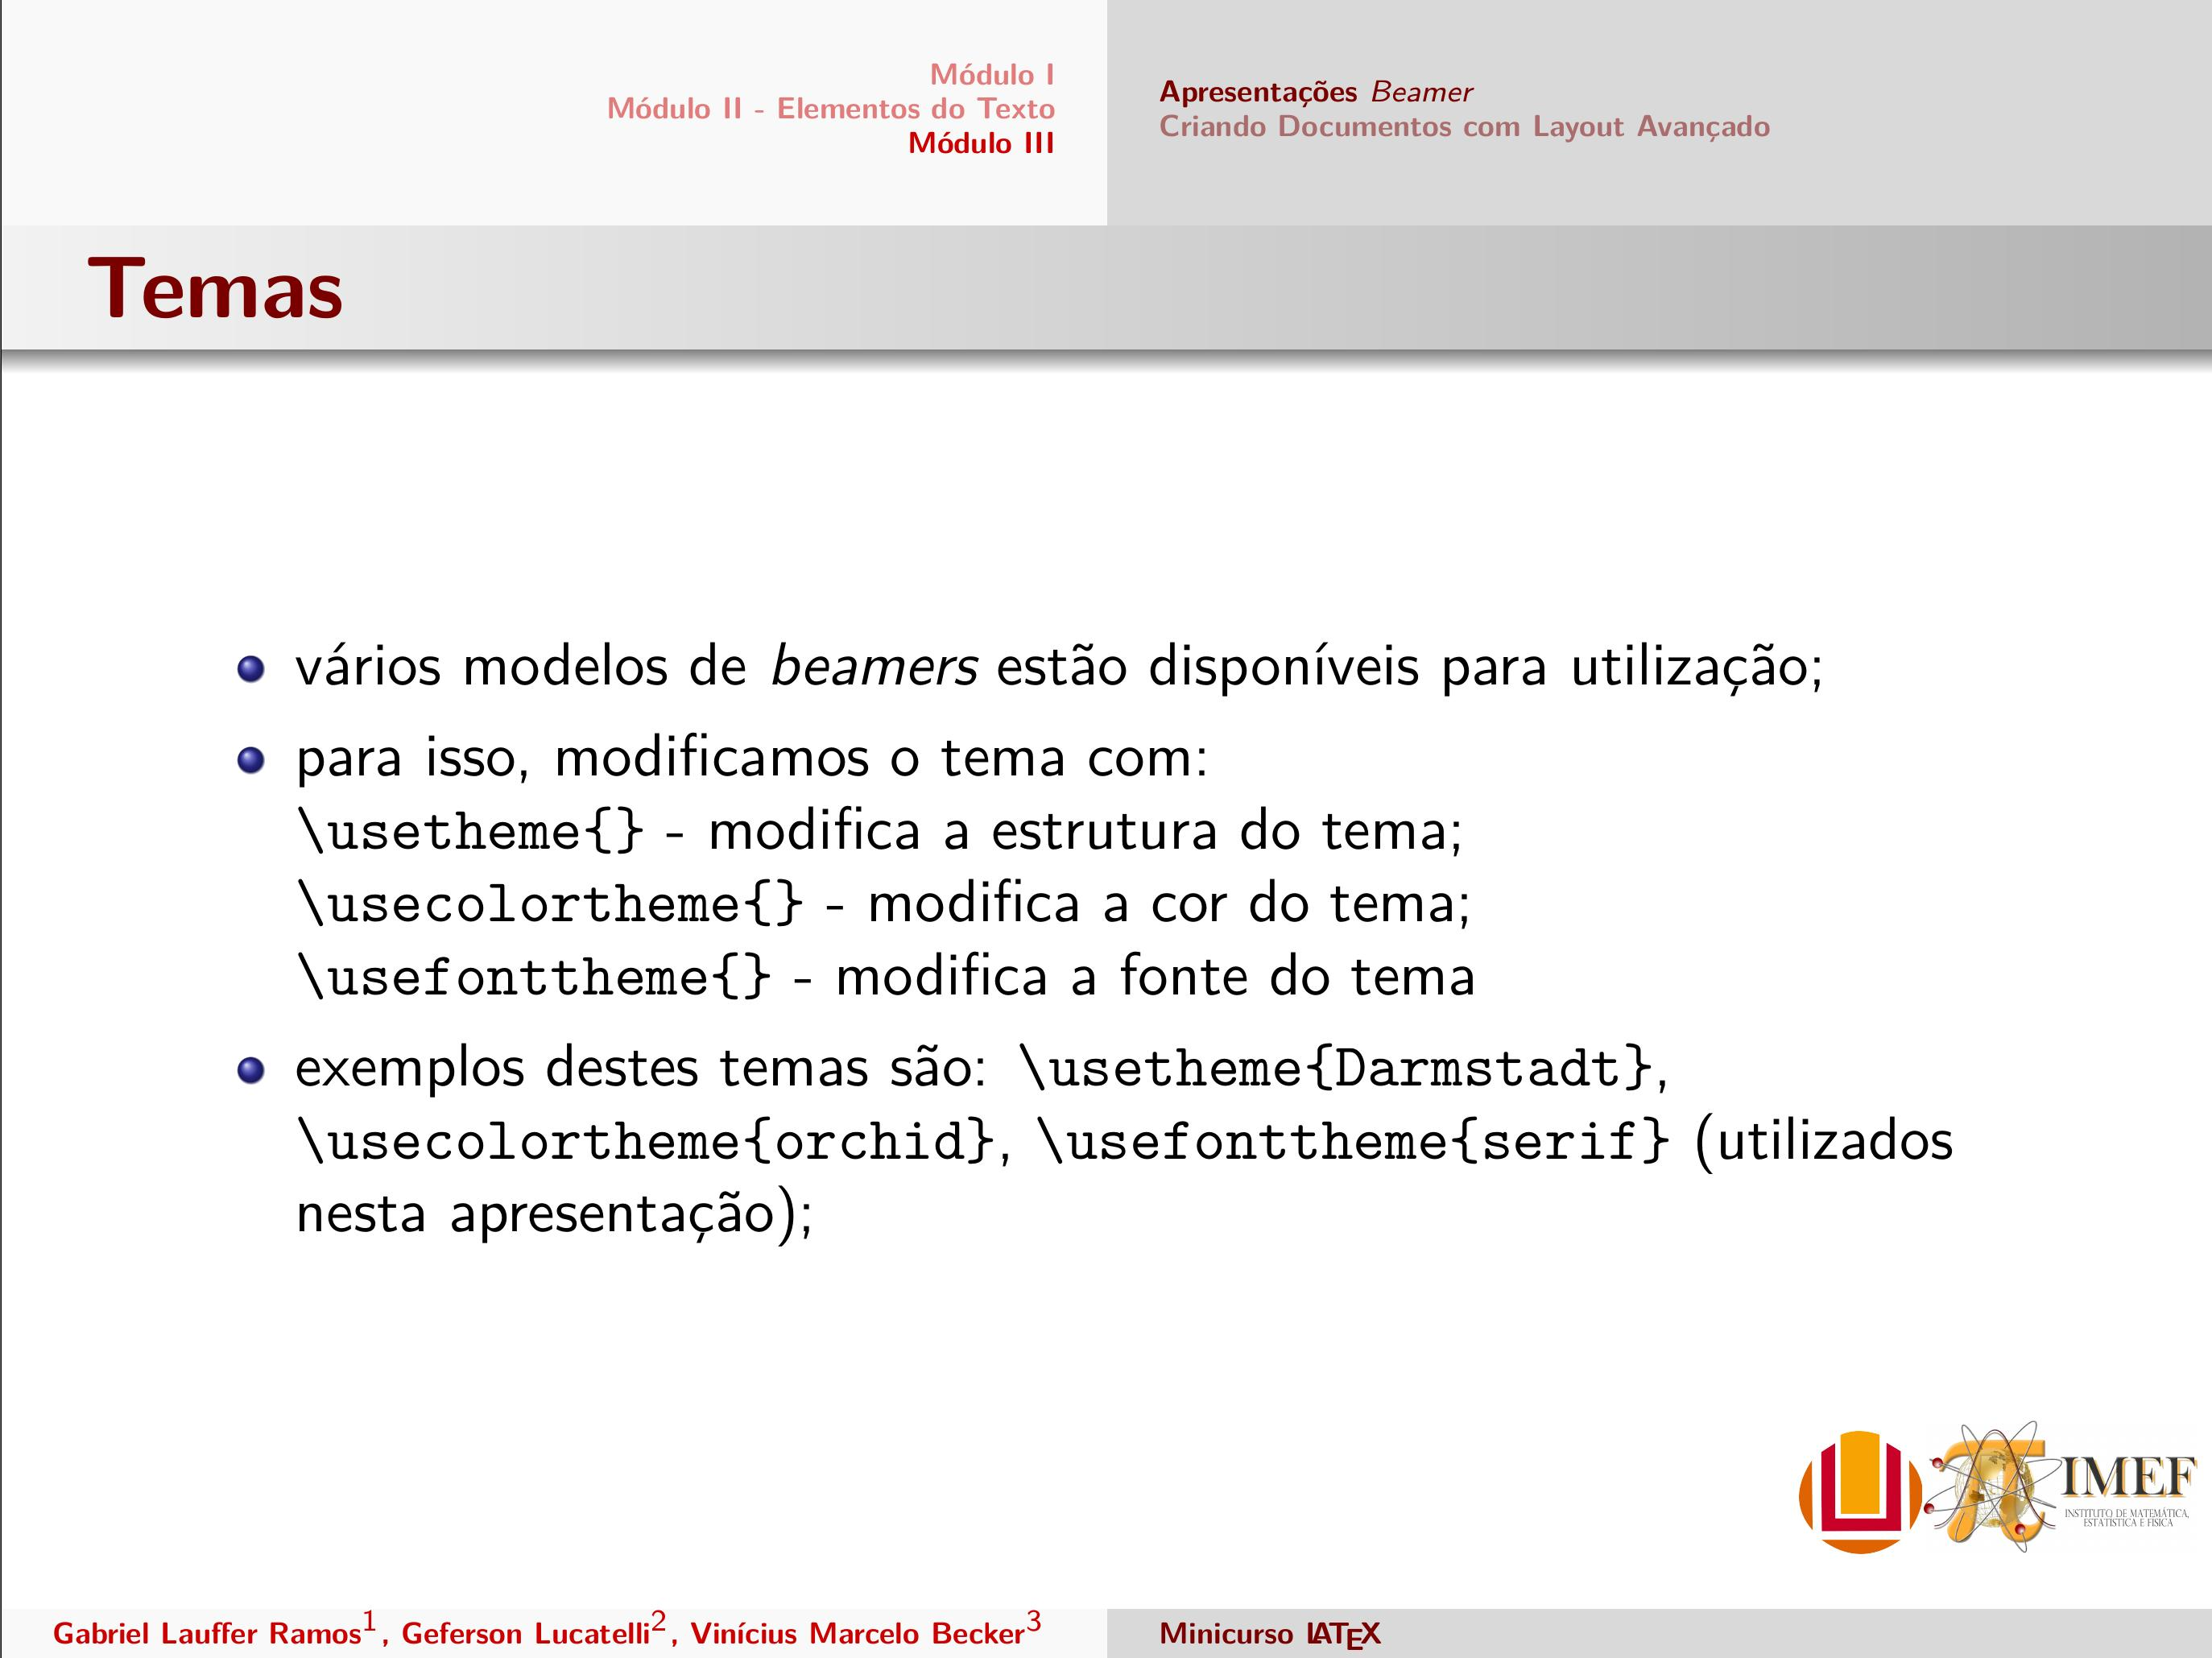
\includegraphics[width=0.40\textwidth]{images/beamer_beav_war.jpg}
\end{figure}
\end{frame}




{\fontsize{5pt}{4.0}\selectfont
\begin{frame}[fragile]{{\sc Temas - este} \texttt{beamer}}
\begin{verbatim}
\documentclass[c]{beamer}
\mode<presentation>
{
\usetheme[progressbar=frametitle]{metropolis}
\usecolortheme{default
\usefonttheme{serif}
\setbeamertemplate{navigation symbols}{}
\setbeamertemplate{caption}[numbered]
\setbeamercovered{transparent}
} 

\usepackage[utf8]{inputenc}
\usepackage[brazil]{babel}
\usefonttheme{serif}
\usepackage{ebgaramond-maths}
\usepackage{amsmath,amssymb}
\usepackage{graphicx}
\usepackage{float}
\usepackage{caption}
\usepackage{subcaption}
\captionsetup[figure]{labelfont=sc}
\usepackage{multicol}
\usepackage{verbatim}

\title{{\sc Introdução ao \LaTeX}}
\subtitle{Módulo 3: Apresentações de slides, Referências e outras técnicas.}
\date{\today}
\author{	{\large XI Semana Acadêmica da Física}\\
Geferson {\sc Lucatelli}\inst{1}\footnote{\texttt{gefersonlucatelli@gmail.com}},
Fernanda Vanucci {\sc Sica}\inst{1}\footnote{\texttt{fervanucci@gmail.com.com\\[0.5cm]}}}
\institute{{\Large Universidade Federal do Rio Grande} \\[0.3cm]
{\inst{1}\large Instituto de Matemática, Estatística e Física
}}
\titlegraphic{\hfill

\includegraphics[height=1.5cm]{images/furg.png}\\[2.5cm]{
\hspace*{8cm}
\includegraphics[height=1.5cm]{images/imef2.png}}
\hspace*{8.5cm}
\includegraphics[height=2.0cm]{images/safis_logo.jpg}
}

\setbeamertemplate{section in toc}{\hspace*{1em}\inserttocsectionnumber.~\inserttocsection\par}
\setbeamertemplate{subsection in toc}{\hspace*{2em}\inserttocsectionnumber.\inserttocsubsectionnumber.~\inserttocsubsection\par}

\begin{document}
\maketitle
\end{verbatim}
\end{frame}
}

\section{Referências}
\plain{Lidando com referências}

\plain{Fazer juntos no Texstudio!}

%\begin{frame}[fragile]{\sc Referências}
%	\begin{itemize}
%		\setlength\itemsep{0.3cm}
%		\item 
%	\end{itemize}
%\end{frame}


\section{Artigos}


\plain{Como personalizar textos em formatos de artigo?}

\begin{frame}[fragile,c]{\sc Artigos}
\begin{itemize}
		\item como já vimos, um artigo é definido basicamente por:
		\begin{verbatim}
		\documentclass[12pt,a4paper]{article}
		\end{verbatim}
		\item usando o pacote \verb|geometry| podemos personalizar as margens do documento:
		\begin{verbatim}
		\usepackage{geometry}
		\geometry{
		a4paper,
		left=20mm,
		top=20mm,
		bottom=20mm,
		right=20mm}
		\end{verbatim}
\end{itemize}
\end{frame}

\begin{frame}[fragile]{\sc Artigos}
Um exemplo de código que permite personalizar o título é: 
{\fontsize{7pt}{6.0}\selectfont
\begin{verbatim}
\title{{\fontsize	{16pt}{10.0}\selectfont  Minicurso \LaTeX}\\
{\fontsize{12pt}{10.0}\selectfont  XI Safis.} \\
\lH{0.07cm}}
\author{\sc Nome Sobrenome$^{\dagger}$}
\date{}	
\maketitle

\begin{center}
(Artigo submetido para ...) \\[2mm]
${^\dagger}$Instituto de Matemática, Estatística e Física - Imef \\
Universidade Federal do Rio Grande - FURG, Rio Grande/RS, Brasil \\
\texttt{\url{e-mail@mail.com}}
%	\date{\today}
\end{center}
\end{verbatim}
}
\end{frame}

\begin{frame}[fragile]{\sc Artigos}
O resultado é:
\begin{figure}[h]
	\centering
	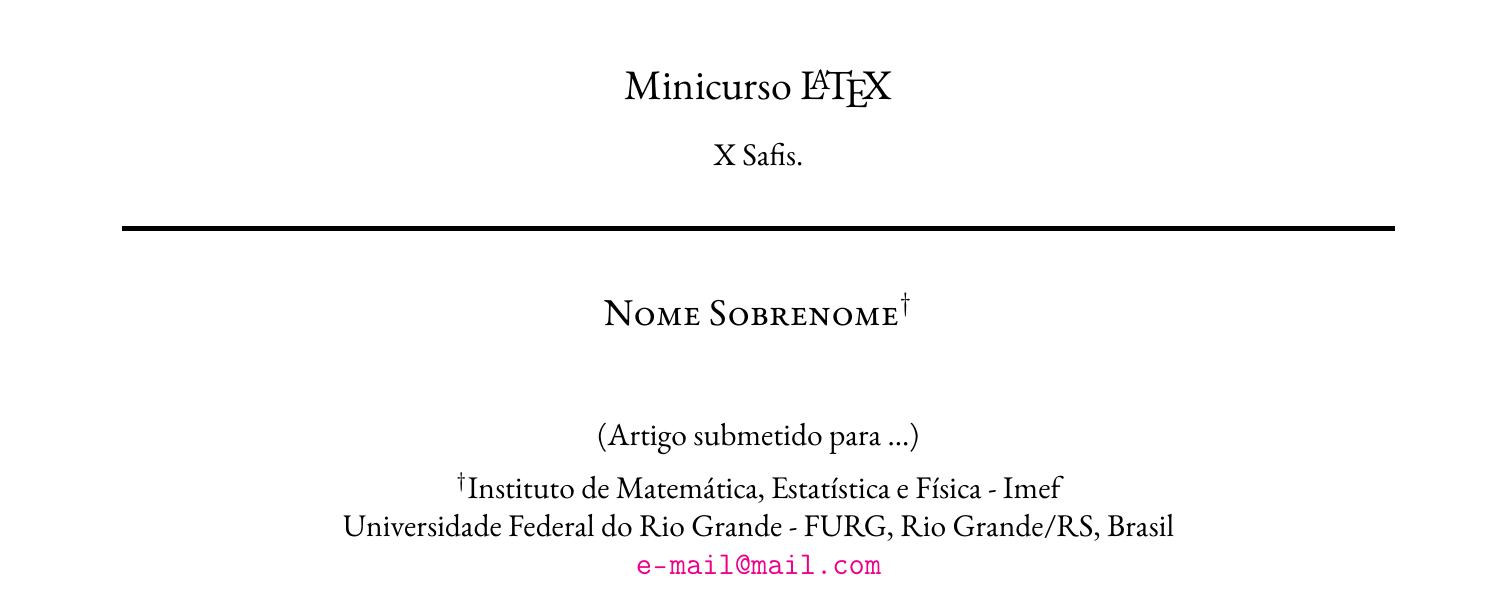
\includegraphics[width=0.99\textwidth]{images/exemp_tit.jpg}
\end{figure}
\end{frame}




\begin{frame}[fragile]{Artigos}
	\begin{itemize}
		\setlength\itemsep{0.3cm}
		\item o pacote \verb|\usepackage{fancyhdr}| configura os \emph{headers} e \emph{footers};
		\item usamos os comandos \verb|\fancyhead[opção]{texto}|, \verb|\fancyfoot[opção]{text}|;
		\item esses comandos são definidos logo após \verb|\usepackage{fancyhdr}|;
		\item por exemplo,
	\end{itemize}
	\begin{exampleblock}{Cabeçalho e Rodapé}
		{\fontsize{7pt}{6.0}\selectfont
			\begin{verbatim}
			\usepackage{fancyhdr}
			\pagestyle{fancy}
			\fancyhead{}\fancyfoot{}
			\fancyhead[C]{titulo title $\bullet$ Maio 2016 $\bullet$ Vol. IX, No. 1} 
			\fancyhead[R]{Jornal...}
			\fancyfoot[RO,LE]{\thepage}
			\end{verbatim}
		}
	\end{exampleblock}
	
	\begin{center}
		
\includegraphics[width=0.80\textwidth]{images/headers_fot.jpg}
	\end{center}
\end{frame}


\begin{frame}[fragile]{\sc Artigos}
	\begin{itemize}
		\item vamos ver agora o que fica no ambiente \verb|document|;
		\item o \verb|abstract| é o ambiente usado para escrever o resumo do artigo:
		\verb|\begin{abstract}|\\
		$\vdots$\\
		\verb|\end{abstract}|
		\item artigos podem ser escritos em uma ou duas colunas (e até mais);
		\item uma das opções na classe artigo é o número de colunas: \verb|onecolumn|, \verb|twocolumn|;
	\end{itemize}
	
\end{frame}




\begin{frame}[fragile]{Artigos}
	\begin{itemize}
		\setlength\itemsep{0.3cm}
		\item uma das grandes vantagens em \LaTeX\ é que muitas revistas de publicações disponibilizam as configurações para 
		a estrutura do texto;
		\item basta apenas adquirir o arquivo e escrever seu artigo;
		\item para a revista \emph{Elsevier}, geralmente suas configurações já estão incluídas nos pacotes instalados,
		e basta apenas usar \verb|\documentclass[review]{elsarticle}|;
		\item outras revistas como o \emph{The Astrophysical Journal}, \emph{MNRAS} e o \emph{The Astronomical Journal} também disponibilizam os formatos;
		\item geralmente é preciso adquirir o arquivo \verb|.cls| de configuração das mesmas;
		\item por exemplo para o Jornal \emph{MNRAS} pode-se usar \verb|\documentclass[a4paper]{mnras}| com este arquivo;
	\end{itemize}
	
\end{frame}



\plain{Fazer no compilador!}

\section{Livros}

\plain{Como preparar textos em formato de livros e teses?}
\begin{frame}[fragile]{\sc Livros e teses}
	\begin{itemize}
		\setlength\itemsep{0.3cm}
		\item vamos verificar primeiramente como construir um modelo de tese ou livro (são semelhantes em estrutura);
		\item mesmo sendo uma tese, usamos a classe \verb|book| com algumas opções:\\
		\verb|\documentclass[a4paper,10pt]{book}|
		\item a estrutura é simples, e adicionamos elementos na medida que queremos;
		\item começaremos com a construção de uma capa;
		\item para isso usa-se o ambiente \verb|titlepage|:\\
		\verb|\begin{titlepage}|\\
		$\vdots$ \\
		\verb|\end{titlepage}|
		\item este deve estar no ambiente \verb|document|;
	\end{itemize}
\end{frame}





\begin{frame}[fragile]{\sc Livros e teses}
	\begin{itemize}
		\setlength\itemsep{0.3cm}
		\item no ambiente \verb|titlepage| informações que podem ser incluídas de imediado como já vimos são: \verb|\title{}|,  \verb|\author{}| e  \verb|\date{}|;
		\item podem repitir a mesma seção de título usada para o artigo;
	\end{itemize}
\end{frame}



\begin{frame}[fragile]{Livros e Teses}{Frontmatter e Mainmatter}
	\begin{itemize}
		\setlength\itemsep{0.3cm}
		\item outros elementos podem adicionados a capa, se desejado;
		\item dando sequência, outras configurações são: agradecimentos, frase do autor, contra capa, \emph{abstract}, etc..
		\item geralmente esses elementos fazem parte da parte \verb|frontmatter| do documento;
		\item isto vai da capa até o sumário;
		\item o restante do documento é parte do \verb|\mainmatter|;
		\item a diferença entre ambos é a criação do sumário, enumeração das páginas: em romano para a primeira e decimal para a segunda, e páginas 
		em branco;
	\end{itemize}
\end{frame}





\begin{frame}[fragile]{Livros e Teses}
	\begin{itemize}
		\setlength\itemsep{0.3cm}
		\item supomos que queiramos adicionar um ambiente \verb|Agradecimentos|, em forma de capítulo mas que não esteja enumerado, e que 
		entre no sumário;
		\item usamos simplesmente \verb|\chapter*{Agradecimentos}|;
		\item um exemplo de como criar tal ambiente é:
		
		\begin{exampleblock}{Seção Agradecimentos}
			\begin{verbatim}
			\chapter*{Agradecimentos}
			\addcontentsline{toc}{chapter}{Agradecimentos}
			\thispagestyle{empty}
			
			Seus agracimentos....
			\clearpage
			\end{verbatim}
		\end{exampleblock}
		
	\end{itemize}
	
\end{frame}

\begin{frame}[fragile]{Livros e Teses}{Frontmatter}
	\begin{itemize}
		\setlength\itemsep{0.3cm}
		\item \verb|\addcontentsline{toc}{chapter}{Agradecimentos}| adiciona Agradecimentos ao sumário (opção \verb|toc|) como se fosse um capítulo (\verb|chapter|), 
		mas na parte  \verb|\frontmatter| enumerada em romanos;
		\item os comandos \verb|\clearpage| ou \verb|\thispagestyle{empty}| removem qualquer outro conteúdo da página;
		\item para adicionar alguma frase ou algo semelhante depois da seção Agradecimentos, deixando uma página em branco, 
		usea apenas o comando \verb|\cleardoublepage| após \verb|\clearpage|, juntamente com \verb|\cleardoublepage|;
	\end{itemize}
	\begin{exampleblock}{Exemplo}
		{\fontsize{8pt}{6.0}\selectfont
			\begin{verbatim}
			\vspace*{0.2\textheight}
			\begin{flushright}
			\noindent "\emph{ sua frase }" \bigbreak
			\hfill seu Nome
			\end{flushright}
			\end{verbatim}
		}
	\end{exampleblock}
	
\end{frame}

\begin{frame}[fragile]{Livros e Teses}{Frontmatter: $Abstract$}
	\begin{itemize}
		\setlength\itemsep{0.3cm}
		\item geralmente, em documentos deste tipo, páginas em branco não são enumeradas;
		\item para remover a enumeração, use após cada \verb|\clearpage| a opção \verb|\thispagestyle{empty}|;
		\item o próximo item é o \emph{abstract} (resumo);
		\item seu ambiente em modelo na classe \verb|book| não existem, mas podemos criá-lo da mesma forma que um artigo:\\
		\verb|\begin{abstract}|\\
		$\vdots$\\
		\verb|\end{abstract}|
		\item usamos o comando \verb|\newenvironment|;
	\end{itemize}
	
\end{frame}


\begin{frame}[fragile]{Livros e Teses}{Frontmatter}
	\begin{itemize}
		\setlength\itemsep{0.3cm}
		\item este comando recebe \verb|\newenvironment{nam}{begdef}{enddef}|;
		\item seu nome \verb|name|, o início da definição \verb|begdef| e o seu fim \verb|enddef|;
		\item chamamos esse ambiente com \verb|\begin{nam}| $\hdots$ \verb|\end{nam}|;
		\item o texto escrito entre o ambiente se adequará a sua definição;
	\end{itemize}
\end{frame}



\begin{frame}[fragile]{Livros e Teses}
Criando ambiante:
		{\fontsize{8pt}{6.0}\selectfont
			\begin{verbatim}
\newenvironment{abstract1}{
\thispagestyle{empty}
\begin{center}
\bigskip
{\huge\textit{Abstract} \par}
\bigskip
\end{center}}
			\end{verbatim}
		}
	Note que é possível colocar o que quiser dentro do novo ambiente.
\end{frame}

\begin{frame}[fragile]{Livros e Teses}{Frontmatter}
	\begin{itemize}
		\setlength\itemsep{0.3cm}
		\item Um resumo dentro do ambiente criado anteriormente fica:
		\begin{verbatim}
		\begin{abstract1}
		Este modelo de tese em \LaTeX\ foi desenvolvido 
		para o Minicurso "Introdução ao \LaTeX\ " na 
		Semana Acadêmica da Física. 
		\end{abstract1}
		\end{verbatim}
		produz:
	\end{itemize}
	\begin{center}
		
\includegraphics[width=0.70\textwidth]{images/abs.jpg}
		% \captionof{figure}{}
	\end{center}
\end{frame}

\begin{frame}[fragile]{Livros e Teses}{Frontmatter}
	\begin{itemize}
		\setlength\itemsep{0.3cm}
%		\item comandos como \verb|\null| e \verb|\vfil| podem ser usados para acomodar a posição do que estará no novo ambiente;
%		\item use-os na definição do ambiente;
		\item usando agora \verb|\tableofcontents| temos:
		\begin{center}
			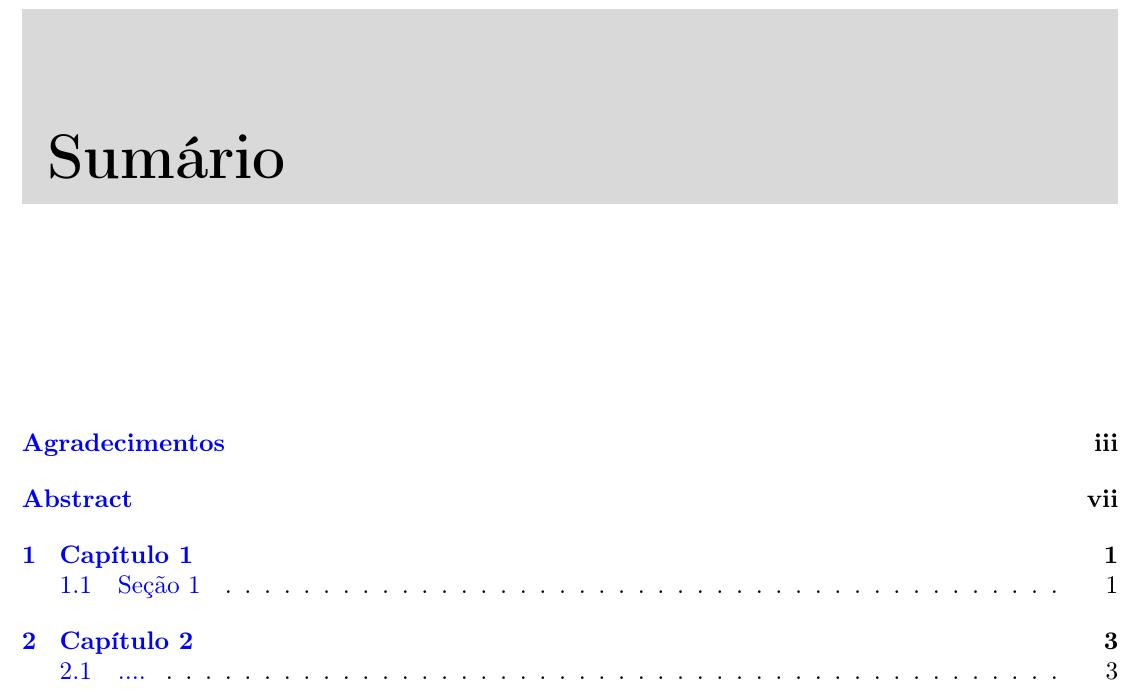
\includegraphics[width=0.60\textwidth]{images/contents.jpg}
			% \captionof{figure}{}
		\end{center}
		\item o uso de \verb|\listoffigures| e \verb|\listoftables| cria sumários referentes a tabelas e figuras;
	\end{itemize}
\end{frame}


\begin{frame}[fragile]{Livros e Teses}{Mainmatter}
	\begin{itemize}
		\setlength\itemsep{0.3cm}
		\item depois do uso do que foi feito anteriormente, usamos \verb|mainmatter| (depois de \verb|\tableofcontents|) para dar início ao conteúdo do 
		documento;
		\item \verb|\chapter{}|, \verb|\section{}|, etc;
		\item o efeito acizentado no título "Sumário" é modificado com o pacote \verb|fncychap|:\\
		\verb|\usepackage[opções]{fncychap}|
		\item dentre as opções temos: \verb|Sonny, Conny, Lenny, Glenn, Renje, Bjarne, Bjornstrup|;
	\end{itemize}
	
\end{frame}

\begin{frame}[fragile]{Livros e Teses}{Mainmatter}
	Exemplos:
	\begin{center}
		
\includegraphics[width=0.60\textwidth]{images/chap_1.jpg}\\
		
\includegraphics[width=0.60\textwidth]{images/chap_2.jpg}\\
		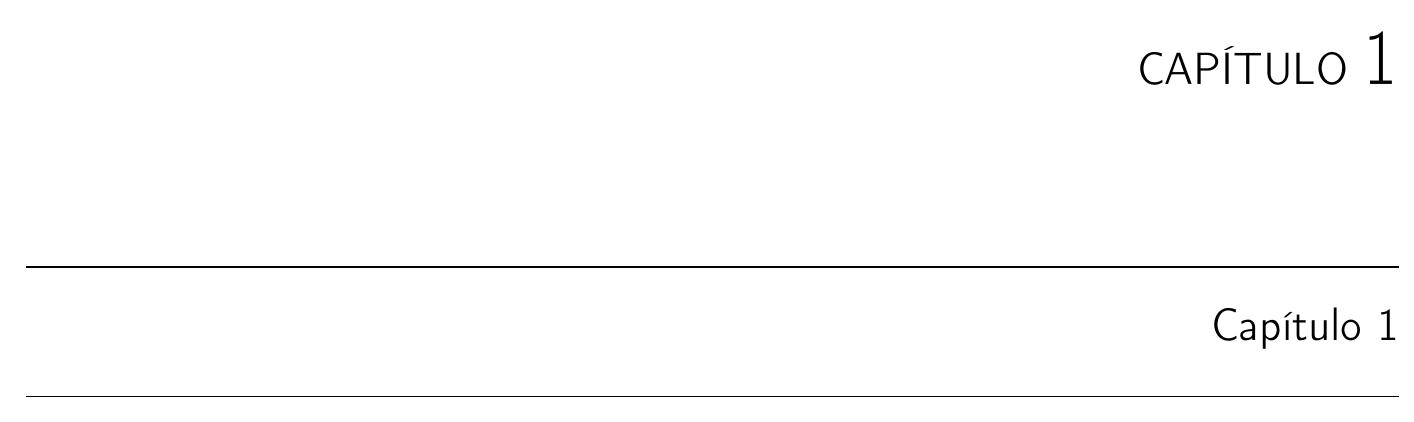
\includegraphics[width=0.60\textwidth]{images/chap_3.jpg}
	\end{center}
\end{frame}


\begin{frame}[fragile]{Livros e Teses}{Mainmatter: apêndice}
	\begin{itemize}
		\setlength\itemsep{0.3cm}
		\item por fim vejamos como construir um apêndice;
		\item usamos o comando \verb|\appendix|: este comando não inclui nenhum apêndice no sumário;
		\item para incluir estes no sumário, usamos logo abaixo de \verb|\appendix|:\\
		\verb|\addcontentsline{toc}{part}{\appendixname}|
		\item \verb|\appendixname| é por definição a palavra "Apêndice" na língua em que está configurado o documento;
		\item depois disso, um apêndice é incluído normalmente por \verb|\chapter{}| (não use o \verb|*|);
	\end{itemize}
\end{frame}



\section{Poster}

\begin{frame}[fragile]{Pôster}{Estrutura e Corpo}
	\begin{itemize}
		\setlength\itemsep{0.3cm}
		\item a classe \verb|a0poster| nos permite criar pôsteres;
		\item inserimos os pacotes que iremos usar e é só começar a criar o pôster;
		\item em um pôster, geralmente não se usa os comandos já prontos como \verb|\title{}|, \verb|\author{}| etc; 
		\item é mais adequando inserir estes no ambiente \verb|\document| com o uso do ambiente \verb|\minipage|;
	\end{itemize}
	
\end{frame}

\begin{frame}[fragile]{Pôster}{Estrutura e Corpo}
	Um exemplo de como fazer isso é:
	\begin{exampleblock}{Informações de um Pôster}
		{\fontsize{8pt}{6.0}\selectfont
			\begin{verbatim}
			\begin{minipage}[b]{0.74\linewidth}
			\veryHuge \color{NavyBlue} \textbf{título} \color{Black}\\
			\Huge\textit{subtítulo}\\[2cm]
			\huge \textbf{autor}\\[0.5cm]
			\huge Universidade Federal do Rio Grande\\[0.4cm] 
			\Large Instituto de Matemática, Estatística e Física\\[0.4cm]
			\Large \texttt{e-mail@e-mail.com}\\
			\end{minipage}
			
			{\vspace{-9cm}\hspace{50cm}{
			\begin{minipage}[b]{0.25\linewidth}
			
\includegraphics[width=6cm]{furg.png}
			
\includegraphics[width=13cm]{imef.jpg}
			\end{minipage}}
			}
			\end{verbatim}
		}
	\end{exampleblock}
	
\end{frame}

\begin{frame}[fragile]{Pôster}{Estrutura e Corpo}
	\begin{itemize}
		\setlength\itemsep{0.3cm}
		\item um pôster pode ser constituído de uma, duas ou três colunas; 
		\item para criar as colunas, usa-se o pacote \verb|multicol|/
		\item após a inclusão do pacote os comandos \verb|\columnsep| \verb|\columnseprule| são usados 
		para configurar as colunas;
		\item \verb|\columnsep=tamanho|: modifica a distância entre as duas colunas;
		\item \verb|\columnseprule=tamanho|: inclui uma linha preta que separa as duas colunas, e \verb|tamanho| indica a grossura da linha;
		\item o ambiente \verb|\abstract| já está definido;
		\item o restante do documento, é construído de forma idêntica as outras classes;
	\end{itemize}
\end{frame}

\begin{frame}[fragile]{Pôster}{Estrutura e Corpo}
	\begin{center}
		
\includegraphics[width=0.99\textwidth]{images/poster.jpg}
	\end{center}
\end{frame}

\plain{Definindo comandos}



\begin{frame}[fragile]{\sc Definindo comandos}
				\begin{itemize}
					\setlength\itemsep{0.3cm}
					\item usamos \verb|\newcommand{cmd}[args]{def}|;
					\item a variável \verb|cmd| é o nome do comando a ser chamado;
					\item \verb|args| é quantos argumentos estão atribuídos ao comando;
					\item \verb|def| é o que o comando irá fazer;
				\end{itemize}
\end{frame}


\begin{frame}[fragile]{\sc Definindo comandos: Exemplo}
	\begin{itemize}
		\setlength\itemsep{0.3cm}
		\item um efeito pode ser adicionado para acomodar o título do trabalho com o instituto e universidade, por exemplo, linhas horizontais;
		\item definimos então: \verb|\newcommand{\linesH}[1]{\rule{\linewidth}{#1}}|, em que \verb|1#| é a grossura da linha;
		\item este comando produz:\\
		\linesH{0.01cm}
		\linesH{0.05cm}
		\linesH{0.1cm}
	\end{itemize}
	
\end{frame}

\plain{Pacote Tikz}


\begin{frame}[fragile]{\LaTeX\ Sources}
	\begin{itemize}
		\setlength\itemsep{0.3cm}
		\item o mundo \LaTeX\ é bastante vasto,
		\item recomendamos à todos o acesso a principalmente quatro fontes que nos auxiliam na construção de documentos \LaTeX:
		\begin{enumerate}
			\item Google (\url{https://www.google.com});
			\item Overleaf (\url{https://www.overleaf.com/});
			\item Tex (\url{http://tex.stackexchange.com/});
			\item ShareLaTeX (\url{https://www.sharelatex.com});
		\end{enumerate}
		
	\end{itemize}
	
\end{frame}





%\begin{frame}[fragile]{{\sc Estrutura do }\texttt{beamer}}
%	\begin{itemize}
%		\setlength\itemsep{0.3cm}
%		\item 
%	\end{itemize}
%\end{frame}
%\section{Referências}



\begin{frame}[allowframebreaks]{References}
\bibliography{references}
\nocite{*}
\end{frame}
\plain{Gracie!}

} 

\end{document}


